\documentclass[]{report}
\usepackage{graphicx}
\usepackage[a4paper,top=1.5cm, left=2cm,right=2cm]{geometry}
\usepackage{listings}
\usepackage{float}
\usepackage{amsmath}
\usepackage{url}
\title{Big data computing - Homework 1}
\author{Giulia Muscarà 1743261}
\date{December 10, 2020} 
\renewcommand{\bibname}{References}

\begin{document}
\maketitle


\section*{Assignment 1}
Locality Sensitive Hashing analyses pairs of signatures likely to be from similar items by taking as input a signature matrix M with m rows. After hashing columns of M to many buckets, each pair of documents that is hashed to the same bucket can be considered a candidate pair. In particular, Locality Sensitive Hashing for Jaccard similarity adopts Jaccard distance as its distance measure. The Jaccard distance of two sets $X$ and $Y$ is computed as $1 - sim(X, Y) = 1 - |X \cap Y|/|X \cup Y|$.\\
As requested, it is assumed that two sets $X$ and $Y$ are considered "similar" or a true positive pair if $Jaccard(X,Y) \ge \theta_{1}$ and that they are a true negative pair if $Jaccard(X,Y) \le \theta_{2}$.\\
It is also assumed that the adopted hash functions behave like an ideal, min-wise independent family, a family of hash functions such that for any
set of arguments $X$ and $x \in X$, the probability that the value of a random function from that family on $x$ will be the smallest among all values of that function on $X$ is about $1/X$.\\
The matrix M is divided into $b$ bands of $r$ rows, implying that $m = r \times b$. For each band, its portion of each column is hashed to a hash table of buckets. Candidate column pairs are those that hash to the same bucket for at least one band. \\
The probability that two pairs with the Jaccard similarity of $t$ are a candidate pair equals to $1 – (1 – t^{r})^{b}$. $B$ and $r$ can be tuned to find most similar pairs, balancing false positives and false negatives. False positives are dissimilar pairs which are hashed to the same bucket and false negatives are similar pairs which are hashed to the different buckets. \\ 
Figure 1 shows the probability curve in the case there is only one threshold to consider, and the curve in the case two thresholds $\theta_{1}$ and $\theta_{2}$ are considered, highlighting the areas corresponding to the probability of missclassifying samples into false positives or false negatives, regardless of what happens in the interval $[\theta_{2}, \theta_{1})$.\\
\begin{figure}[h]
	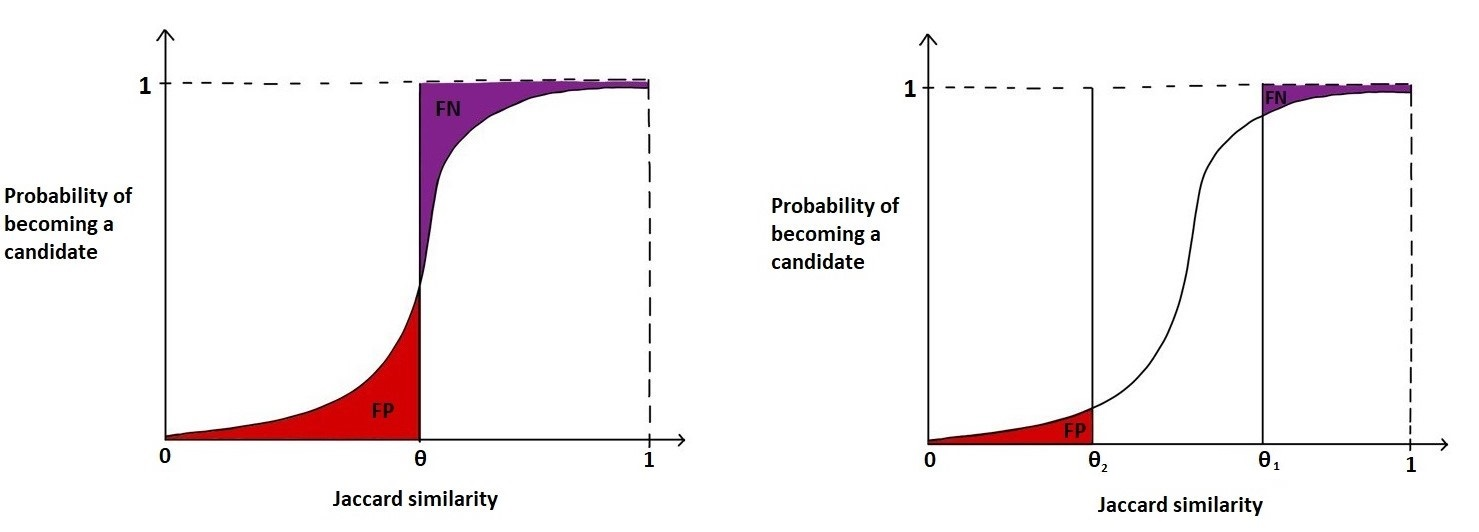
\includegraphics[width=1\textwidth]{grafici_fp_fn.jpg}
	\caption{S-curve with one and two thresholds}
\end{figure}\\
False positive probability is represented by the red area. Indeed, the pairs with $Jaccard(X,Y) \le \theta_{2}$ falling under the S-curve must not be considered a candidate pair because of the threshold imposition. In the same way false negative probability is represented by the violet area because pairs with $Jaccard(X,Y) \ge \theta_{1}$ that are above the curve should be considered a candidate pair, given the threshold imposition.\\
To write $FPP$ and $FNP$ in function of $b, r$ and of the tresholds, their respective areas can be computed with the use of integrals \cite{fpfn}. $FPP$ is given by the area under the curve between $0$ and $\theta_{2}$, while the latter by the difference between area of the right side rectangle and the area below the curve in the interval $[\theta_{1}, 1)$.\\
$$
FNP = 1 \times \theta_1 - \int_{\theta_1}^{1} 1 - (1 - t^r)^b dt = 1 \times \theta_1 - F(1) + F(\theta_1)
$$
$$
FPP = \int_{0}^{\theta_2} 1 - (1 - t^r)^b dt = F(\theta_2) - F(0) = F(\theta_2) 
$$
To compute $F(t)$, the S-curve can be integrated using the Newton Binomial as follows.\\
$$
(a+b)^n = \sum_{k=0}^{n} \binom{n}{k} a^{n-k} b^k\
(1-t^r)^b = \sum_{p=0}^{b} (-1)^p \binom{b}{p} 1^{b-p} t^{rp}
$$
$$
F(t) = \int 1-(1-t^r)^b dt = \int dt - \int \sum_{p=0}^{b} (-1)^p \binom{b}{p}t^{rp} dt = t - \sum_{p=0}^{b} (-1)^p \binom{b}{p}\int t^{rp} dt =\
= t - \sum_{p=0}^{b} (-1)^p \binom{b}{p}\frac{1}{rp + 1}t^{rp+1}
$$
It can be concluded that $FNP = \theta_1 - 1 + \sum_{p=0}^{b} (-1)^p \binom{b}{p}\frac{1}{rp + 1} + \theta_{1} - \sum_{p=0}^{b} (-1)^p \binom{b}{p}\frac{\theta_1^{rp+1}}{rp + 1} \le p_1 $ and that $FPP = \theta_2 - \sum_{p=0}^{b} (-1)^p \binom{b}{p}\frac{\theta_2^{rp+1}}{rp + 1} \le p_2$. Given the constants $\theta_{1}$, $\theta_{2}$, $p_1$ and $p_2$, $r$ and $b$ can be adjusted to minimize false positive and false negative probabilities and must be chosen such that $m = r \times b$. There may be several suitable pairs of $r$ and $b$ values, but in the case that m is too small, it may happen that no pair exists such that it satisfies at the same time the disequations and the imposition $m = r \times b$. A higher value of b implies a higher probability of finding candidate pairs and of false positives, viceversa is b is too small, there will be a higher number of false negatives.\\
In the worst cases, false positive probability will be maximised if $b = m$ and $r = 1$, as the curve will be a concave function, while false negative probability will be maximised if $b = 1$ and $r = m$ because the function will be convex \cite{lsh}. The behaviour of the curve in both cases is shown in Figure 2. \\
\begin{figure}[h]
	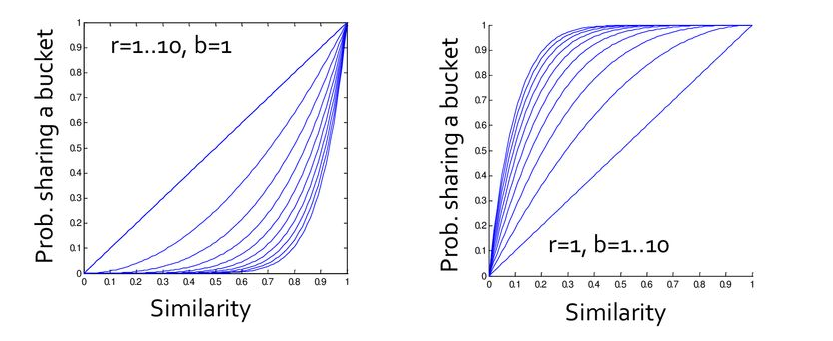
\includegraphics[width=1\textwidth]{worstcases.png}
	\caption{S-curve shape when b=1 or r=1 \cite{image} }
\end{figure}\\
\clearpage


\section*{Assignment 2}
$\bullet$ It is assumed that A is a square-invertible matrix of dimension $n$, with SVD $A = U \Sigma V^T$ = $\sum_{i=1}^{n} \sigma_i u_i v_i^T$. Given that $A$ is square, also $U$ and $V$ will be square matrices of dimension $n$. $\Sigma$ is a diagonal square matrix again of dimension $n$. A's inverse matrix $A^{-1}$ can be computed as follows to prove that it equals to $B = \sum_{i=1}^{n} \frac{1}{\sigma_i} v_i u_i^T$.\\\\
$A^{-1} = (U \Sigma V^T)^{-1} = (V^T)^{-1} \Sigma^{-1} U^{-1}$\\\\
Notice that $U$ is a square and orthogonal matrix because it represents an orthonormal basis in $\Re^n$, so its inverse matrix equals to its transposed \cite{mat}. The same is valid for $V$. Also, because $\Sigma$ is a diagonal matrix, $\Sigma^{-1}$ is again a diagonal matrix with the inverse of the elements of the diagonal of $\Sigma$ on its diagonal.\\
As a consequence, the above formula can be rewritten as:\\\\
$A^{-1} = (V^T)^{-1} \Sigma^{-1} U^{-1} = (V^T)^{T} \Sigma^{-1} U^{T} = V \Sigma^{-1} U^{T} $ \\\\
At the same time $B = \sum_{i=1}^{n} \frac{1}{\sigma_i} v_i u_i^T = V \Sigma^{-1} U^{T}$ , so it can be concluded that $A^{-1} = B$.\\\\
$\bullet$ It is assumed that $A$ is a square matrix of dimension $n$, with SVD $A = U \Sigma V^T$ = $\sum_{i=1}^{r} \sigma_i u_i v_i^T$ but not necessarily invertible. $B = \sum_{i=1}^{r} \frac{1}{\sigma_i} v_i u_i^T$ is the Moore-Penrose inverse of $A$, which is a unique pseudo-inverse that every matrix has. If $A$ was square but not invertible, its pseudo-inverse B would satisfy the properties $ABA = A$ and $BAB = B$, but not $A+A = I$. \\
It can be proved that $BAx = x$, $ \forall x$ $|$ $x = \sum_{i=1}^{r} \alpha_i v_i$, for every vector that can be expressed as a linear combination of the right singular vectors of $A$.\\\\
$BA = (\sum_{i=1}^{r} \frac{1}{\sigma_i} v_i u_i^T)(\sum_{i=1}^{r} \sigma_i u_i v_i^T) = (\frac{1}{\sigma_1} v_1 u_1^T+...+\frac{1}{\sigma_r} v_r u_r^T)(\sigma_1 u_1 v_1^T+...+\sigma_r u_r v_r^T) = \sum_{i=1}^{r} v_i v_i^T$	\\\\
The above equivalence is true because whenever $i \ne j$, $u_i u_j^T = 0$ and $v_i v_j^T = 0$ given that U and V are orthogonal matrices, which means that their columns are orthogonal vectors. Moreover, when $i = j$, $u_i^T u_i = 1$, so the product can be reduced to the above final sum. It can be written that:\\\\
$\forall \space 1 \le k \le r$, $BAv_k = \sum_{i=1}^{r} v_i v_i^T v_k = v_k v_k^T v_k = v_k$\\\\
Indeed, for any $i \ne k$, $v_i^T v_k = 0$ and for $i = k$, $v_i^T v_k = 1$.\\ Hence, $\forall 1 \le k \le r$, $BA \alpha_k v_k = \alpha_k v_k$ and it can be concluded that $BAx = x$ for any $x$ in the span of singular vectors of $A$.
\clearpage

\begin{thebibliography}{9}
	\bibitem{fpfn}
	Hossein and Mahjur, 
	\textit{A Solution for Calculating the False Positive and False Negative in LSH Method to Find Similar Documents},
	Journal of Basic and Applied Scientific Research, TextRoad Publication,
	2013.
	
	\bibitem{lsh}
	Gupta, S.,
	\textit{Locality Sensitive Hashing},
	Towards Data Science,
	\url{https://towardsdatascience.com/understanding-locality-sensitive-hashing-49f6d1f6134},
	2018.
	
	\bibitem{image}
	Leskovec, J.,
	\textit{Mining Massive Datasets},
	Stanford University,
	2011.
	
	\bibitem{mat}
	Vandenberghe, L.,
	\textit{Orthogonal matrices},
	Applied Numerical Computing, UCLA,
	2019.	
	
	
	
\end{thebibliography}
\end{document}      